\chapter{Benchmark Design}
We developed a tool, called StreamBench, to execute benchmark workloads on stream processing systems. A key feature of StreamBench is extensibility, so that it could be extended not only to run new workloads but also to benchmark new stream processing systems. We have used StreamBench to measure the performance of several stream processing systems, as we report in the next chapter.  StreamBench is also available under an open source license, so that others may use and extend it, and contribute new workloads and stream processing system interfaces.

In this chapter, we describe the architecture of StreamBench and introduce more detail of main components of StreamBench. 

\section{Architecture}

\begin{figure}
  \begin{center}
  \subfigure{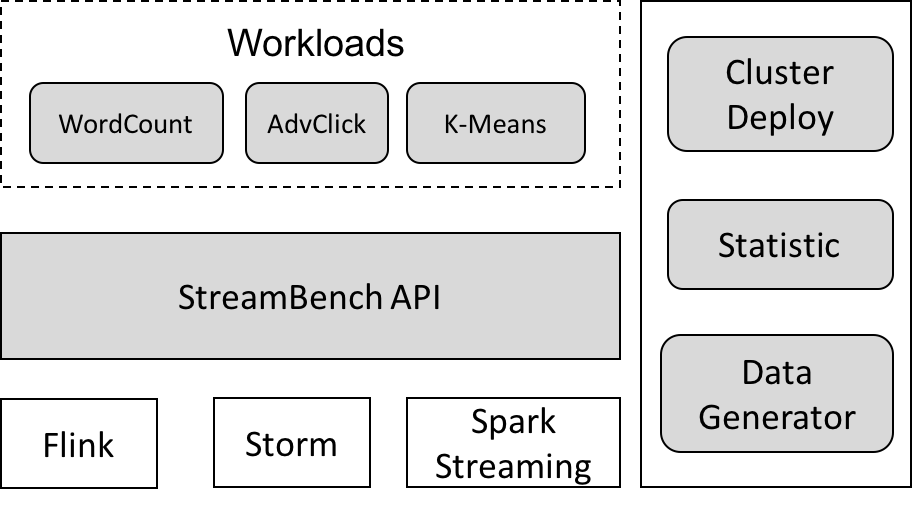
\includegraphics[scale=0.6]{images/benchmark_architecture}}
   \caption{StreamBench architecture}
   \label{fig:streambench_architecture}
  \end{center}
\end{figure}

The main component of StreamBench is a Java program for consuming data from partitioned kafka topic and runs workloads on stream processing cluster. In the program, there is a set of common APIs for stream processing which could be engined by stream processing systems. Currently we support these APIs on three stream processing systems: Storm, Flink and Spark Streaming. Several workloads are implemented by these common APIs. In StreamBench we implemented three workloads to benchmark performance of stream processing systems in different aspects. The architecture of StreamBench is shown in Figure~\ref{fig:streambench_architecture}. 

Except the core Java program, the architecture also includes three more components: Cluster Deploy, Data Generator and Statistic. Section ~\ref{chapter:environment_setup} describes how to use cluster deploy scripts to setup experiment environment. Data generators generate test data for workloads and send it to kafka cluster that is demonstrated detailedly in Section~\ref{section:data_generator}. The Statistic component discussed in Section~\ref{section:log_statistic} includes experiment logging and performance statistic. 

\section{Experiment Environment Setup}
\label{chapter:environment_setup}

\subsection{Hardware}

The experiment environment consists of two clusters: compute cluster and Kafka cluster. Computer cluster consists of 8 work nodes and one master nodes. Kafka cluster has 5 brokers with one zookeeper instance running on the same machine with one Kafka broker. Each above node is a visual machine which has 4 CPU and 15 GB RAM. All the nodes are in the same local area network that provides low latency and high throughput connectivity. 

\subsection{Software}
The operator system running on experiment nodes is Ubuntu 14.04 LTS. Benchmarked stream processing systems are Spark-1.5.1, Storm-0.10.0 and Flink-0.10.1. To enable checkpoint feature of Spark, Hadoop2.6(HDFS) is installed in compute cluster. Kafka 0.8.2.1 is running as distribute message system here. 

To deploy these software in compute cluster and kafka cluster automatically, we developed a set of python script. The prerequisites of using these scripts include internet access, ssh passwordless login between nodes in cluster and cluster configuration that describes which nodes are compute node or kafka node and where is the master node. The basic logic of deploy scripts is to download softwares online and install them, then replace configure files which are contained in a Github repository. For detail information of how to use cluster deploy scripts and configure of Storm, Flink, Spark and Kafka, please check this Github repository~\footnote{\url{https://github.com/wangyangjun/StreamBench}}.

\section{Workloads}
\label{section:workloads}

In StreamBench, a workload consists of a stream processing application and one or more kafka topics. The application consumes messages from kafka cluster and executes operations or transformations on the messages. We have developed 3 workloads to evaluate different aspects of a system's performance. Each workload contains a representative operation or feature of stream processing system that can be used to evaluate systems at one particular point in the performance space. We have not attempted to exhaustively examine the entire performance space. As StreamBench is open sourced, users could also defined their own workloads either by defining a new set of workload parameters, or if necessary by implement a new workload which is discussed detailedly in section~\ref{section:extensibility}.


\subsection{WordCount}

With the widespread use of computer technologies, there is increasing demand of processing unbounded, continuous input streams. In most cases, only basic operations need to be performed on the data streams such as \texttt{map}, \texttt{reduce}. One good sample is stream WordCount. WordCount is a very common sample application of Hadoop MapReduce that counts the number of occurrences of each word in a given input set. \cite{MapReduce} Similarly many stream processing systems also support it as an sample application to count words in a  given input stream. Stream WordCount is implemented with basic operations which are supported by almost all stream processing systems. It means either the system has such operations by default or the operations could be implemented with provided built-in APIs. Other basic operations include \texttt{flatMap}, \texttt{mapToPair} and \texttt{filter} which are similar to \texttt{map} and could be implemented by specializing \texttt{map} if not supported by default. In StreamBench, there are a set of corresponding basic APIs defined. The pseudocode of WordCount implemented with these basic APIs could be abstracted as following:

\begin{lstlisting}
    sentenceStream.flatMap(...)
                  .mapToPair(...)
                  .reduceByKey(...)
                  .updateStateByKey(...);

\end{lstlisting}

One special case of the basic APIs is \texttt{updateStateByKey}. Only in Spark Streaming there is a corresponding built-in operation. As discussed in Section~\ref{section:spark}, the computing model of Spark Streaming is micro-batch which is different with that of other stream processing systems. The results of operation \texttt{reduceByKey} of WordCount running in Spark Streaming is word counts of one single micro batch data set. Operation \texttt{updateStateByKey} is used to accumulate word counts in Spark Streaming. As the model of Flink and Storm is stream processing and accumulated word counts are returned from \texttt{reduceByKey} directly. Therefore, in the implementations of \texttt{updateStateByKey} with Flink and Storm, nothing need to do. The goal of this workload is to evaluate the performance of stream processing systems executing basic operations.  


\subsection{Click Stream}

Besides the cases in which only basic operations need to be performed, another typical type of stream use case is processing joins over unbounded streams. For example, in a surveillance application, we may want to correlate cell phone traffic with email traffic. Theoretically unbounded memory is required to processing join over unbounded input streams, since every record in one infinite stream must be compared with every record in the other. Obviously, this is not practical. \cite{window-join} Since the memory of a machine is limited, we need restrict the number of records stored for each stream. 

Join



\subsection{KMeans}

Iterative 



\section{Data Generators}
\label{section:data_generator}


\section{Experiment Logging and Statistic}
\label{section:log_statistic}
\begin{figure}
  \begin{center}
  \subfigure{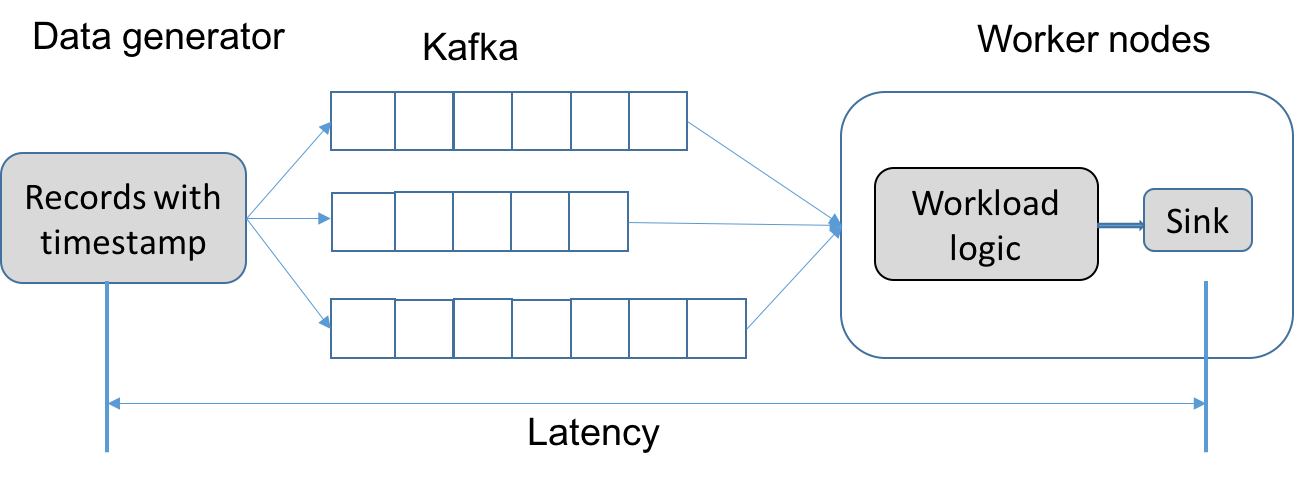
\includegraphics[scale=0.5]{images/latency}}
   \caption{Latency}
   \label{fig:latency}
  \end{center}
\end{figure}

For evaluating the performance, there are two performance measurement terms used in StreamBench that are latency and throughput. Latency is the required time from a record entering the system to some results produced after some actions performed on the record. In StreamBench, messaging system and stream processing system are combined together and treated as one single system. The latency is computed start from when a record is generated. As discussed in Section \ref{section:data_generator}, data is sent to kafka cluster immediately after generation. Figure~\ref{fig:latency} shows how latency computed in StreamBench. 

Throughput is the number of actions executed or results produced per unit of time. In the WordCount workload, throughput is computed as the number of words counted per seconds in the whole compute cluster. Joined clicked stream and the number of points processed per second are the throughput of workloads AdvClick and Stream KMeans respectively.

There is an inherent tradeoff between latency and throughput: on a given hardware setup, as the amount of load increases by increase the speed of data generation, the latency of individual records increases as well since there is more contention for disk, CPU, network, and so on. Computing latency start from records generated makes it easy to measure the highest throughput, since records couldn't produced in time will stay in kafka topics that increase latency dramatically. A stream processing system with better performance will achieve low latency and high throughput with fewer servers.

\section{Extensibility}
\label{section:extensibility}

One significant feature of StreamBench is extensibility. The component "Workloads" in Figure~\ref{fig:streambench_architecture} contains three predefined workloads discussed in Section~\ref{section:workloads} that are implemented with common stream processing APIs. First, with some configuration modification of a data generator, which allows user to vary the skew in record popularity, and the size and number of records. The performances of a workload processing data streams with different properties could be different a lot. Moreover, it is easy for developers to design and implement a new workload to benchmark some specific features of stream processing systems. This approach allows for introducing more complex stream processing logic, and exploring tradeoffs of new stream processing features; but involves greater effort compared to the former approach.

Besides implementing new workloads, StreamBench also could be extended to benchmark new stream processing systems by implement a set of common stream processing APIs. A few samples of APIs could be shown as following:
\begin{itemize}
\item \textbf{map}(MapFunction\textless \textbf{T}, \textbf{R}\textgreater fun, String componentId): map each record in a stream from type \textbf{T} to type \textbf{R}
\item \textbf{mapToPair}(MapPairFunction\textless \textbf{T, K, V}\textgreater fun, String componentId): map a  item stream\textbf{\textless T\textgreater } to a pair stream\textbf{\textless K, V\textgreater}
\item \textbf{reduceByKey}(ReduceFunction\textless \textbf{V}\textgreater fun, String componentId): called on a pair stream of (\textbf{K, V}) pairs, return a new pair stream of (\textbf{K, V}) pairs where the values for each key are aggregated using the given reduce function
\end{itemize}

These methods are quite simple, representing common data transformations. There are some other APIs like \texttt{filter()}, \texttt{flatMap()} and \texttt{join} which are also easily to implement and supported well by most stream processing systems. Despite its simplicity, this API maps well to the native APIs of many of the stream processing systems we examined.





